\documentclass[slides]{pgnotes}

\title{Markdown}

\begin{document}

\maketitle

\tableofcontents

\section{Documentation examples}

A research data analyst conducts computational studies on the effects of seismic activity on marine bird migration patterns.
Their code is primarily Python and C++ interacting with SQL databases and API feeds from data providers.
The institute additionally releases their code as open source for others to use.
They produce documentation: 

\begin{itemize}

\item
  \textbf{Scientific paper(s)} on the software's theory, algorithms, performance and limitations.
  
\item
  \textbf{README} file for those wishing to use the software and install it (and its dependencies).

\item
  \textbf{Manuals} for those using the software on a day-to-day basis

\end{itemize}

\textbf{What format should these be in?}


\section{Word Processors}

\subsection{Limitations}

\begin{description}

\item[Binary format:] word processor files are binary (not text format):
  \begin{itemize}
  \item Must use original / compatible program
  \item Difficult to automate
  \item Cannot use text manipulation tools (e.g. \texttt{diff})
  \item Limits usefulness and performance of source control
  \end{itemize}
\item[Platform limitations:] cannot use from all platforms (e.g. Linux server)
\item[Usability:] ``helpful'' auto-correct can corrupt technical content!
  
\end{description}


\subsection{Alternatives}

\textbf{Use a plain text format (.txt)}
\begin{description}
\item[Program independent:] use any text editor
  \begin{itemize}
  \item Use within your coding IDE!
  \end{itemize}
\item[Small file size] compared to equivalent \texttt{.docx}.
\item[Text-based tools] like \texttt{diff} work.
\item[Source control] can show version changes. 
\item[Convert easily] to PDF, HTML, EPUB, etc.
\end{description}


\section{Markdown}

\begin{center}
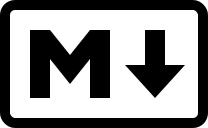
\includegraphics[width=0.25\linewidth]{markdown_logo}
\end{center}

\begin{quotation}
  ``Markdown is a lightweight markup language for creating formatted text using a plain-text editor. John Gruber and Aaron Swartz created Markdown in 2004 as a markup language that is intended to be easy to read in its source code form. Markdown is widely used for blogging and instant messaging, and also used elsewhere in online forums, collaborative software, documentation pages, and readme files.'' --- Wikipedia
\end{quotation}

\href{https://spec.commonmark.org/0.30/}{CommonMark specification}

\subsection{Basic document sample (sample.md)}

\inputminted{markdown}{sample.md}

\subsection{Conversions}

\begin{center}
\includegraphics[width=0.9\linewidth]{md_conversions}
\end{center}

\end{document}
